% !TeX encoding = windows-1251
\documentclass[a4paper,11pt]{article}

\usepackage{newlistok}
\usepackage{tikz}
\УвеличитьШирину{2cm}
\УвеличитьВысоту{2.5cm}
%\vspace*{1.0cm}

\newcommand{\har}{\mathop{\mathrm{char}}\nolimits}
\renewcommand{\spacer}{}

\renewcommand{\C}{{\mathbb C}}
\newcommand{\Zp}{{\mathbb Z}_p}
\renewcommand{\Z}{\mathbb Z}
\renewcommand{\Q}{\mathbb Q}
\renewcommand{\R}{\mathbb{R}}
%\newcommand{\QT}{{\Q[\sqrt{\raisebox{0ex}[1.35ex]{$2$}}]}}
\newcommand{\QT}{\Q[\sqrt{2}]}
\newcommand*{\longermapsto}{\mathop{\mapstochar\relbar\mskip-10.5mu\rightarrow}}


\newcommand{\ci}{^{\circ}}
\newcommand{\s}{\sin}
\renewcommand{\r}{\sqrt}
\renewcommand{\f}[2]{\left(\frac{#1}{#2}\right)}
\newcommand{\sk}[1]{\left({#1}\right)}
\newcommand{\fr}{\frac}
\renewcommand{\c}{\cos}
\renewcommand{\t}{\tg}
\newcommand{\ct}{\ctg}
\renewcommand{\a}{\alpha}
\renewcommand{\b}{\beta}
\newcommand{\e}{\epsilon}
\newcommand{\w}{\widetilde}
\newcommand{\g}{\gamma}
\renewcommand{\d}{\dfrac}
\renewcommand{\le}{\leqslant}
\renewcommand{\ge}{\geqslant}
\renewcommand{\phi}{\varphi}
\renewcommand{\l}[2]{\log_{#1}#2}
\newcommand{\sns}{\mskip-.5mu}

%\renewcommand*{\hm}[1]{#1\nobreak\discretionary{}%
%{\hbox{$\mathsurround=0pt #1$}}{}}
%

\newcommand{\regionB}[1]
{   \fill[#1] (30:2) arc (60:0:{2*sqrt(3)}) arc (-60:120:{2*sqrt(3)}) arc (60:0:{2*sqrt(3)});
}

\newcommand{\regionBB}[1]
{   \fill[#1] (270:2) arc (-120:120:{2*sqrt(3)}) arc (60:-60:{2*sqrt(3)});
}

\newcommand{\regionAA}[1]
{   \fill[#1] (270:2) arc (240:120:{2*sqrt(3)}) arc (60:300:{2*sqrt(3)});
}

\newcommand{\regionAABB}[1]
{   \fill[#1] (270:2) arc (-60:60:{2*sqrt(3)}) arc (120:240:{2*sqrt(3)});
}


\newcommand{\regionA}[1]
{   \fill[#1] (150:2) arc (180:120:{2*sqrt(3)}) arc (60:240:{2*sqrt(3)}) arc (180:120:{2*sqrt(3)});
}

\newcommand{\regionC}[1]
{   \fill[#1] (270:2) arc (240:300:{2*sqrt(3)}) arc (360:180:{2*sqrt(3)}) arc (240:300:{2*sqrt(3)});
}

\newcommand{\regionAB}[1]
{   \fill[#1] (30:2) arc (0:60:{2*sqrt(3)}) arc (120:180:{2*sqrt(3)}) arc (120:60:{2*sqrt(3)});
}

\newcommand{\regionBC}[1]
{   \fill[#1] (30:2) arc (60:0:{2*sqrt(3)}) arc (300:240:{2*sqrt(3)}) arc (-60:0:{2*sqrt(3)});
}

\newcommand{\regionAC}[1]
{   \fill[#1] (150:2) arc (120:180:{2*sqrt(3)}) arc (240:300:{2*sqrt(3)}) arc (240:180:{2*sqrt(3)});
}

\newcommand{\regionABC}[1]
{   \fill[#1] (30:2) arc (60:120:{2*sqrt(3)}) arc (180:240:{2*sqrt(3)}) arc (-60:0:{2*sqrt(3)});
}

\newcommand{\regionDarkside}[1]
{   \fill[#1,even odd rule] (270:2) arc (-120:120:{2*sqrt(3)}) arc (60:300:{2*sqrt(3)}) (-7,-7) rectangle (7,7);
}

\newcommand{\mycolor}{blue!50!cyan}
\newcommand{\mynocolor}{white}


\begin{document}

\НомерЛистка{11}
\Заголовок{Логика}
\ДатаЛистка{04.2014}

\СоздатьЗаголовок

%\выдд{Основные обозначения}

$a\in A$ --- элемент $a$ принадлежит множеству $A$, например, $2\in \N$.

$a\not\in A$ --- элемент $a$ не принадлежит множеству $A$, например $-5 \not \in \N$

$A \subset B$ --- $A$ является подмножеством $B$ (все элементы $A$ принадлежат $B$ ), например $\{1,2,3\} \subset \{1,2,3,4,5\}.$

$\emptyset$ --- пустое множество.

$A \cap B$ --- пересечение множеств $A$ и $B$ (множество всех элементов, принадлежащих $A$ и $B$).

$A \cup B$ --- объединение множеств $A$ и $B$  (множество всех элементов, принадлежащих либо $A$, либо $B$).

$A \backslash B$ --- разность множеств $A$ и $B$ (множество всех элементов, принадлежащих $A$, но не принадлежащих $B$).

\задача Часто множества изображают в виде кругов на
плоскости (диаграммы Эйлера-Венна). Посмотрите на следующие
диаграммы Эйлера-Венна и запишите, каким множествам
соответствуют заштрихованные области. Для записи используйте
символы $\cup$, $\cap$, $\backslash$ и скобки.
\кзадача

 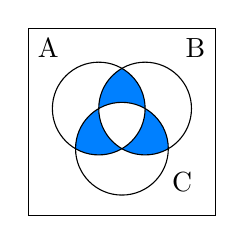
\begin{tikzpicture}[scale=0.17]

 \regionA{\mynocolor} \regionB{\mynocolor} \regionC{\mynocolor}
 \regionAB{\mycolor} \regionAC{\mycolor}\regionBC{\mycolor}
 \regionABC{\mynocolor}
   \draw (30:2) circle ({2*sqrt(3)});
   \draw (150:2) circle ({2*sqrt(3)});
   \draw (270:2) circle ({2*sqrt(3)});
   \draw (-5.5,5.5) node {A};
   \draw (4.5,-4.5) node {C};
   \draw (5.5,5.5) node {B};
    \draw (-7,-7) rectangle (7,7);

 \end{tikzpicture} \quad
  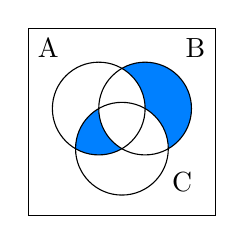
\begin{tikzpicture}[scale=0.17]

 \regionA{\mynocolor} \regionB{\mycolor} \regionC{\mynocolor}
 \regionAB{\mynocolor} \regionAC{\mycolor}\regionBC{\mynocolor}
 \regionABC{\mynocolor}
   \draw (30:2) circle ({2*sqrt(3)});
   \draw (150:2) circle ({2*sqrt(3)});
   \draw (270:2) circle ({2*sqrt(3)});
   \draw (-5.5,5.5) node {A};
   \draw (4.5,-4.5) node {C};
   \draw (5.5,5.5) node {B};
    \draw (-7,-7) rectangle (7,7);

 \end{tikzpicture} \quad 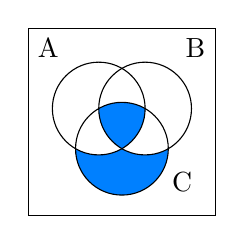
\begin{tikzpicture}[scale=0.17]

 \regionA{\mynocolor} \regionB{\mynocolor} \regionC{\mycolor}
 \regionAB{\mynocolor} \regionAC{\mynocolor}\regionBC{\mynocolor}
 \regionABC{\mycolor}
   \draw (30:2) circle ({2*sqrt(3)});
   \draw (150:2) circle ({2*sqrt(3)});
   \draw (270:2) circle ({2*sqrt(3)});
   \draw (-5.5,5.5) node {A};
   \draw (4.5,-4.5) node {C};
   \draw (5.5,5.5) node {B};
    \draw (-7,-7) rectangle (7,7);

 \end{tikzpicture}\quad 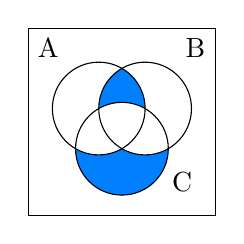
\begin{tikzpicture}[scale=0.17]

 \regionA{\mynocolor} \regionB{\mynocolor} \regionC{\mycolor}
 \regionAB{\mycolor} \regionAC{\mynocolor}\regionBC{\mynocolor}
 \regionABC{\mynocolor}
   \draw (30:2) circle ({2*sqrt(3)});
   \draw (150:2) circle ({2*sqrt(3)});
   \draw (270:2) circle ({2*sqrt(3)});
   \draw (-5.5,5.5) node {A};
   \draw (4.5,-4.5) node {C};
   \draw (5.5,5.5) node {B};
    \draw (-7,-7) rectangle (7,7);

 \end{tikzpicture} \quad 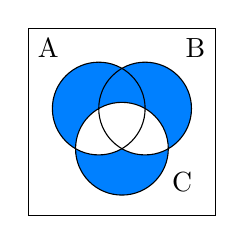
\begin{tikzpicture}[scale=0.17]

 \regionA{\mycolor} \regionB{\mycolor} \regionC{\mycolor}
 \regionAB{\mycolor} \regionAC{\mynocolor}\regionBC{\mynocolor}
 \regionABC{\mynocolor}
   \draw (30:2) circle ({2*sqrt(3)});
   \draw (150:2) circle ({2*sqrt(3)});
   \draw (270:2) circle ({2*sqrt(3)});
   \draw (-5.5,5.5) node {A};
   \draw (4.5,-4.5) node {C};
   \draw (5.5,5.5) node {B};
    \draw (-7,-7) rectangle (7,7);

 \end{tikzpicture} \quad 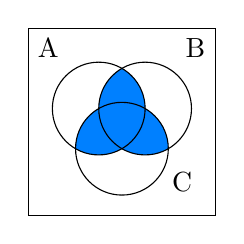
\begin{tikzpicture}[scale=0.17]

 \regionA{\mynocolor} \regionB{\mynocolor} \regionC{\mynocolor}
 \regionAB{\mycolor} \regionAC{\mycolor}\regionBC{\mycolor}
 \regionABC{\mycolor}
   \draw (30:2) circle ({2*sqrt(3)});
   \draw (150:2) circle ({2*sqrt(3)});
   \draw (270:2) circle ({2*sqrt(3)});
   \draw (-5.5,5.5) node {A};
   \draw (4.5,-4.5) node {C};
   \draw (5.5,5.5) node {B};
    \draw (-7,-7) rectangle (7,7);

 \end{tikzpicture}

\задача Каждый третий политик – бизнесмен, а каждый
четвертый бизнесмен – политик. Кого больше, политиков или
бизнесменов?
\кзадача

\задача Пусть , $A=\{2k+1,k\in \Z\}$, $B=\{3k,k\in \Z\}$.
($A$ --- нечетные, $B$ --- делящиеся на 3). Найдите пересечение $A\cap B$ и
разность $B\backslash A$.
\кзадача

\задача Число $x$ натуральное. Среди утверждений 1) $2x>70$,
2) $x<100$, 3) $3x>25$, 4) $x \ge 10$, 5) $x>5$ три
верных и два неверных. Чему равно $x$?
\кзадача

\задача Перед футбольным матчем команд  <<Север>>  и <<Юг>> было дано пять прогнозов:
1) ничьей не будет; 2) в ворота <<Юга>> забьют; 3) <<Север>> выиграет; 4) <<Север>> не проиграет; 5) в матче будет забито ровно $3$ гола. После матча выяснилось, что верными оказались ровно три прогноза. С каким счётом закончился матч?
\кзадача

\задача Расставьте вместо многоточий слова «необходимо», «достаточно», и там, где это возможно, «необходимо и достаточно» так, чтобы получились верные суждения.\\
\пункт Для того, чтобы число $x$ делилось на $5$, $\ldots$, чтобы его десятичная запись кончалась цифрой $0$.\\
\пункт Для того, чтобы число $x$ делилось на $9$, $\ldots$, чтобы сумма цифр его десятичной записи делилась на $3$.\\
\пункт Для того, чтобы параллелограмм $ABCD$ был ромбом, $\ldots$, чтобы его диагонали делили пополам внутренние~углы.
\пункт Для того, чтобы параллелограмм $ABCD$ был квадратом, $\ldots$, чтобы его стороны были равны.
\кзадача


\опр Будем говорить, что утверждение $\overline{P_1}$ является \выд{отрицанием} к утверждению $P_1$, если $\overline{P_1}$ верно тогда и только тогда, когда не верно $P_1$.
\копр

\задача Покажите, что если из $P_1$ следует $P_2$, то это равносильно тому, что из $\overline{P_2}$ следует $\overline{P_1}$ .
\кзадача

\задача Докажите, что если $m >1$ и $(m-1)! + 1$ делится на $m$, то число $m$ --- простое.
\кзадача

\задача Равносильны ли утверждения «кто не с нами, тот против нас» и «кто не против нас, тот с нами»?
\кзадача

\задача Рассмотрим утверждения вида «$P_1$ и $P_2$» (обозначается $P_1 \wedge P_2$ ) и «$P_1$ или $P_2$» (обозначается $P_1 \vee P_2$).
Докажите следующие теоремы (правила де Моргана):

\пункт Утверждение $\overline{P_1 \wedge P_2}$ равносильно $\overline{P_1} \vee\overline{P_2}$;
\пункт Утверждение $\overline{P_1 \vee P_2}$ равносильно $\overline{P_1} \wedge \overline{P_2}$.
\кзадача

\задача Однажды принцесса сказала: «Хочу, чтобы мой муж был красивый, не был глупым или некрасивым, или чтобы был некрасивым, но не был глупым». Упростите данное утверждение.
\кзадача

\задача Рассмотрим утверждения вида «для любого $h\in H$ верно $Q$» (обозначается $\forall h\in H : Q$) и «существует $h\in H$ такой, что верно $Q$» (обозначается $\exists h\in H : Q$). Постройте отрицания к этим утверждениям.
\кзадача

\задача Постройте отрицание к утверждению «для любого четырехугольника существует вписанная в него окружность» и покажите, что оно истинно.
\кзадача

\задача В квадрате $3 \times 3$ закрашено $5$ клеток. Докажите, что найдется закрашенная клетка, в строке и в столбце которой найдется еще по одной закрашенной клетке.
\кзадача

\задача Постройте отрицания к следующим утверждениям:

\пункт В каждом классе найдется ученик, который решил хотя бы одну задачу из контрольной.

\пункт Найдется класс, в котором каждый ученик решил хотя бы одну задачу из контрольной.

\пункт Существует такая задача, что в каждом классе хотя бы один ученик ее решил.

\пункт Для каждой задачи есть класс, в котором все ученики ее решили.

\пункт Есть город, в каждом районе которого есть улица, на которой в каждом доме есть однокомнатная квартира.

\пункт В каждом городе есть магазин, в котором нет хлеба, и никто из продавцов не знает, когда он будет.

\кзадача

\задача Попытайтесь формализовать фразу «ученики должны показывать свои тетради учителям», рассматривая множества учеников, тетрадок и учителей. Придумайте несколько вариантов, как это можно сделать. \кзадача

\ЛичныйКондуит{0.2mm}{7mm}
%\СделатьКондуит{8mm}{7mm}




\end{document} 